\subsubsectionwithauthor[author={Mika Landeck},email={mika.landeck@fau.de}]{Aufgabe 4: NP-Vollständigkeit}

\paragraph{(a)}
	Dazu wird das Vorgehen einer nichtdeterministischen Zweiband-TM skizziert, welche das Problem im Polynomieller Zeit lößt:
	\begin{enumerate}
		\item Überprüfe, ob $w$ von der Form $c(V,E,k)$ ist mit $(V,E)$ repräsentiert einen Graphen $G$ und $k \in \mathbb{N}$ (auf Band 1).
		\item Wähle nichtdeterministisch einen Knoten $v'$ aus $V$ und füge ihn der Knotenmenge $V'$ hinzu (kodiert auf Band 2).
		\item Überprüfe, ob es zu $v'$ ein $v''$ in $V'$ gibt, sodass $(v',v'')\in E$ liegt (auf Band 2). \begin{itemize}
			\item Falls es kein solches $v''$ in $V'$ gibt, wiederhole ab Schritt 2.
			\item Falls genau ein solches $v''$ in $V'$ existiert und $|V'|\geq k$ gilt, halte und akzeptiere.
			\item Falls mehrere Kandidaten für $v''$ in $V'$ gefunden werden und $|V'|-1\geq k$ gilt, halte und akzeptiere.
			\item Falls mehrere Kandidaten für $v''$ in $V'$ gefunden werden und $|V'|-1 < k$ gilt, halte und akzeptiere \underline{nicht}.
		\end{itemize}
	\end{enumerate}
	\textit{Anmerkung: Durch die nichtdeterministische Wahl wird stets das passende $v'$ hinzugefügt, falls ein solches existiert (Vorstellung vom allwissenden Orakel).}

	\textbf{Laufzeitanalyse:} Der Syntaxcheck in Schritt 1 läut mit nichtdeterministischem Raten der Übergänge im Eingabewort von $V$ nach $E$ und nach $k$ in $O(|V|)+O(|E|)+O(k)\leq O(n)$. Schritt 2 läuft maximal in $O(|V'|)\leq O(|V|)\leq O(n)$. Die erste Überprüfung in Schritt 3 erfordert höchstens $O(|V'|)\cdot O(|E|)\leq O(n^2)$. Die Bestimmung der Mächtigkeit von $V'$ und der Abgleich mit $k$ erfolgen in $O(|V'|)+O(k)\leq O(n)$.\\
	Die Schritte 2 und 3 werden höchstens $|V|$ mal wiederholt. Insgesamt arbeitet die NTM also in $O(n^3)$.

	Daraus folgt, dass das in der Aufgabe beschriebene Graphenproblem in NP liegt.

\paragraph{(b)}
	Sei	$L_1=\{c(V,E,k)\ |\ G=(V,E)\ ist\ Graph \wedge k\in \mathbb{N}: \exists V' \subseteq V:(\nexists e=(v_1,v_2)\in E\ mit\ v_1,v_2 \in V') \wedge |V'|\geq k \}$\\
	die Sprache, deren Wortproblem gleich dem Entscheidungsproblem einer unabhängigen Menge in $G$ ist.

	Sei	$L_2=\{c(V,E,k)\ |\ G=(V,E)\ ist\ Graph \wedge k\in \mathbb{N}: \exists V' \subseteq V:|\{e=(v_1,v_2)\in E\ |\ v_1,v_2 \in V'\}|\leq 1 \wedge |V'|\geq k \}$\\
	die Sprache, deren Wortproblem gleich dem Entscheidungsproblem einer fast unabhängigen Menge mit mindestens $k$ Knoten in $G$ ist.

	Man verwende folgenden Ansatz für die polynomielle Reduktion:\\
	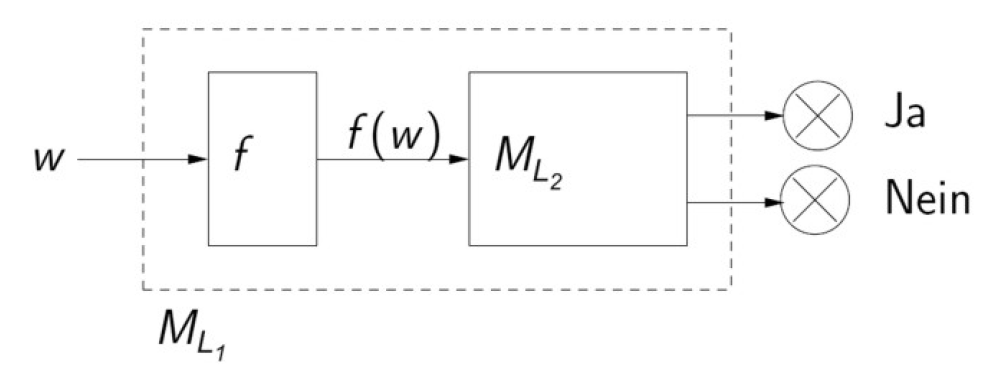
\includegraphics[scale=0.4]{thinf/sol/f23t2/reduction_idee_skizze}

	Dazu wird eine totale und berechenbare Funktion $f$ benötigt, die das Wortproblem aus $L_1$ auf das Wortprobleme aus $L_2$ abbildet:

	Sei $f:L_1 \rightarrow L_2$ definiert über

	$f(w)=\begin{cases}
		c(\tilde{V},\tilde{E},\tilde{k})&\text{falls $w=c(V,E,k)$ mit $G=(V,E)$ ist Graph und $k \in \mathbb{N}$}\\
		\varepsilon &\text{sonst}
	\end{cases}$\\
	Dabei wird $V$ um zwei Knoten $v_1,v_2 \notin V$ ergänzt und zum neuen $\tilde{V}=V\cup \{v_1,v_2\}$. Die neuen Knoten bilden auch eine Kante, somit ist $\tilde{G}=G\cup \{(v_1,v_2)\}$. Außerdem gilt $\tilde{k}=k+2$.

	$f$ ist offensichtlich total. Außerdem lässt sich eine DTM konstruieren, die $f$ in polynomieller Laufzeit berechnet:
	\begin{itemize}
		\item Syntaxcheck, ob $w$ von der Form $c(V,E,k)$ ist, wobei $(V,E)$ einen Graphen $G$ repräsentiert und $k \in \mathbb{N}$ (höchstens in $O(n^2)$).
		\item An die Kodierung von $V$ zwei neue Knoten $v_1$ und $v_2$ anhängen (höchstens in $O(n^2)$).
		\item An die Kodierung von $G$ die neue Kante $(v_1,v_2)$ anhängen (höchstens in $O(n)$).
		\item Zu $k$ in der entsprechenden Kodierung $2$ addieren (höchstens in $O(n)$).
	\end{itemize}

	Es bleibt noch zu zeigen, dass $w \in L_1 \Leftrightarrow f(w) \in L_2$ gilt. Dies beweisen folgende Äquivalenzumformungen ($\forall w \in L_1$):
	\begin{align*}
		w \in L_1 \Leftrightarrow\ & w=c(V,E,k)\ mit\ G=(V,E)\ ist\ Graph\ und\ k \in \mathbb{N}\\
		& \wedge (\exists V'\subseteq V:\nexists e=(v_1,v_2)\in E\ mit\ v_1,v_2 \in V' \wedge |V'|\geq k)\\
		\Leftrightarrow\ &f(w)=c(\tilde{V},\tilde{E},\tilde{k})\ mit\ \tilde{G}=(\tilde{V},\tilde{E})\ ist\ Graph\ und\ \tilde{k} \in \mathbb{N}\\
		& \wedge (\exists V'\subseteq V:\nexists e=(v_1,v_2)\in E\ mit\ v_1,v_2 \in V' \wedge |V'|\geq \tilde{k}-2)\\
		\Leftrightarrow\ &f(w)=c(\tilde{V},\tilde{E},\tilde{k})\ mit\ \tilde{G}=(\tilde{V},\tilde{E})\ ist\ Graph\ und\ \tilde{k} \in \mathbb{N}\\
		& \wedge (\exists \tilde{V'}\subseteq \tilde{V}:\exists! e=(v_1,v_2)\in \tilde{E}\ mit\ v_1,v_2 \in \tilde{V'} \wedge |\tilde{V'}|=|V'|+2\geq \tilde{k})\\
		\Leftrightarrow\ &f(w)=c(\tilde{V},\tilde{E},\tilde{k})\ mit\ \tilde{G}=(\tilde{V},\tilde{E})\ ist\ Graph\ und\ \tilde{k} \in \mathbb{N}\\
		& \wedge (\exists \tilde{V'}\subseteq \tilde{V}: |\{e=(v_1,v_2)\in \tilde{E}\ \vert\ v_1,v_2 \in \tilde{V'}\}|\leq 1 \wedge |\tilde{V'}|\geq \tilde{k})\\
		\Leftrightarrow\ &f(w) \in L_2
	\end{align*}
	\textit{Informelle Beschreibung: Man füge zwei neue Knoten mit einer gemeinsamen Kante hinzu und erhöhe $k$ um $2$. Somit kann für jede unabhängige Menge in $L_1$ mit Mächtigkeit $k$ eine fast unabhängige Menge in $L_2$ mit Mächtigkeit $k+2$ gefunden werden, die zusätzlich genau die neu hinzugefügten Knoten enthält. Falls eine fast unabhängige Menge in $L_2$ nur einen der extra hinzugefügten Knoten enthält, muss eine Kante aus $E$ enthalten sein. Allerdings kann dann einer der Knoten dieser Kante weggelassen werden und es gibt immer noch eine unabhängige Menge in $L_1$ mit zwei Knoten weniger (einer der hinzugefügten und einer aus der Kante). Die Rückrichtung stimmt also auch.}

	Somit gilt $L_1 \leq_p L_2$ und da $L_1$ NP-hart ist, muss $L_2$ auch NP-hart sein, denn die Relation $\leq_p$ ist transitiv. Da $L_2$ zudem in NP liegt (siehe (a)), ist $L_2$ und damit das entsprechende Graphenproblem NP-vollständig.
